\lecture{16}{30. Oktober 2025}{Bending -- Shear and Moment Diagram}

\begin{problemwithimage}{f11_2}{11-2}
  Draw the shear and moment diagrams for the beam.
  \textit{Hint}: The \qty{100}{\kN} load must be replaced by equivalent loadings at point $C$ on the axis of the beam.
\end{problemwithimage}

\begin{derivation}
  We replace the \qty{100}{\kN} load with a corresponding axial load and couple moment.
  This becomes an axial load of
  \begin{equation*}
    P = -\qty{100}{\kN} 
  \end{equation*}
  and a couple moment of
  \begin{equation*}
    M_0 = P \cdot d = \qty{-100}{\kN} \cdot \qty{-0.25}{\m} = \qty{25}{\kN.\m} 
  .\end{equation*}

  Now we just need to find the vertical support reactions.
  Using a force equilibrium we get
  \begin{align*}
    \sum F_y &= 0 \\
    A_y + B_y - \qty{75}{\kN} &= 0 \\
    A_y + B_y &= \qty{75}{\kN} 
  .\end{align*}
  
  And a moment equilibrium yields:
  \begin{align*}
    \sum M_A &= 0 \\
    \qty{3}{\m} \cdot B_y - \qty{75}{\kN} \cdot \qty{1}{\m} + \qty{-25}{\kN.\m} &= 0 \\
    B_y &= \qty{33,33}{\kN} \implies A_y = \qty{41.67}{\kN} 
  .\end{align*}

  This means that our shear diagram can be made based on:
  \begin{itemize}
    \item $0<x<1$: \qty{41,67}{\kN} 
    \item $x = 1$: $\qty{41.67}{\kN} - \qty{75}{\kN} = \qty{-33,33}{\kN}$
    \item $1 < x < 3$: \qty{-33,33}{\kN}
    \item $x = 3$: \qty{0}{\kN} 
  \end{itemize}

  Our moment diagram can be made using $M(0) = 0$ and $\mathrm{d}M / \mathrm{d}x = V$ and the jump from the couple moment $M_0 = \qty{25}{\kN.\m}$.
  This means we get:
  \begin{itemize}
    \item $0 \leq x <  1$: $M(x) = 41.67 x$
    \item $1 \leq x < 2$: $M(x) = 41.67 - 75 (x-1) = 75 - 33.33 x$
    \item $x = 2$: $M(x) = 75 - 33.33 x + 25 = 100 - 33.33 x$
    \item $2 < x < 3$: $M(x) = 100 - 33.33 x$
  \end{itemize}

  \begin{figure} [ht]
    \centering
    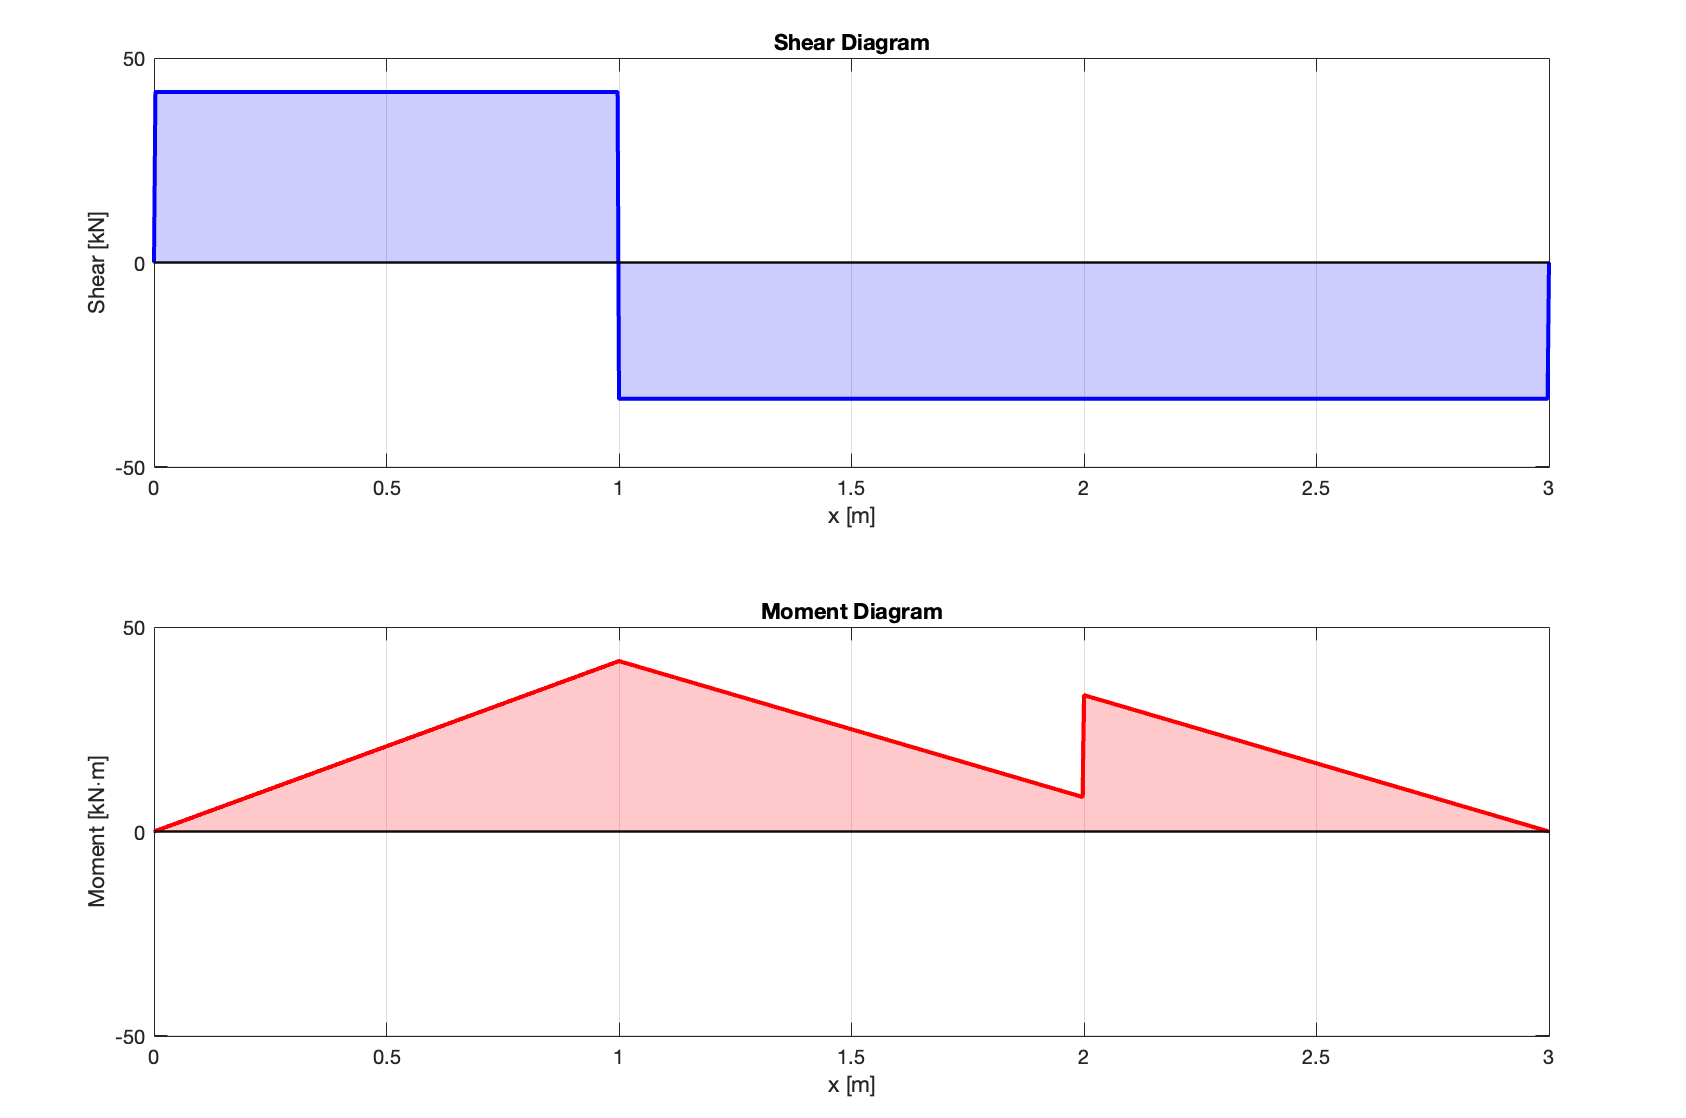
\includegraphics[width=\linewidth]{./figures/f11_2sm.png}
    \caption{Shear and moment diagrams for the beam.}
  \end{figure}
\end{derivation}

\clearpage

\begin{problemwithimage}{f11_18}{11-18}
  Draw the shear and moment diagrams for the simply supported beam.
\end{problemwithimage}

\begin{derivation}
  We start by finding the vertical support reactions.
  First we use the force equilibrium:
  \begin{align*}
    \sum F_y &= 0 \\
    A_y + B_y - \qty{4}{\kN} &= 0 \\
    A_y + B_y &= \qty{4}{\kN}
  .\end{align*}
  And then the moment equilibrium:
  \begin{align*}
    \sum M_A &= 0 \\
    - \qty{2}{\kN.\m} - \qty{4}{\kN} \cdot \qty{4}{\m} + B_y \cdot \qty{6}{\m} &= 0 \\
    B_y &= \frac{\qty{2}{\kN.\m} + \qty{4}{\kN} \cdot \qty{4}{\m}}{\qty{6}{\m}}\\
    B_y &= \qty{3}{\kN}  \\
    A_y &= \qty{1}{\kN} 
  .\end{align*}
  This means that our piecewise defined shear diagram is given by:
  \begin{itemize}
    \item $0<x \leq 2$: $V(x) = \qty{1}{\kN}$
    \item $2 \leq x < 4$: $V(x) = \qty{1}{\kN}$
    \item $x = 4$: $V(x) = - \qty{3}{\kN}$
    \item $4 \leq x <6$: $V(x) = \qty{-3}{\kN}$
  \end{itemize}

  And our moment diagram is then:
  \begin{itemize}
    \item $0 < x < 2$: $M(x) = x$
    \item $x = 2$: $M(2-) = 2 \implies M(2+) = 2 + 2 = 4$
    \item $2 < x < 4$: $M(x) = 4 + 1(x-2) = x + 2 \implies M(4) = 6$
    \item $4 < x < 6$: $M(x) = 6 - 3(x-4)$.
  \end{itemize}

  \begin{figure} [ht]
    \centering
    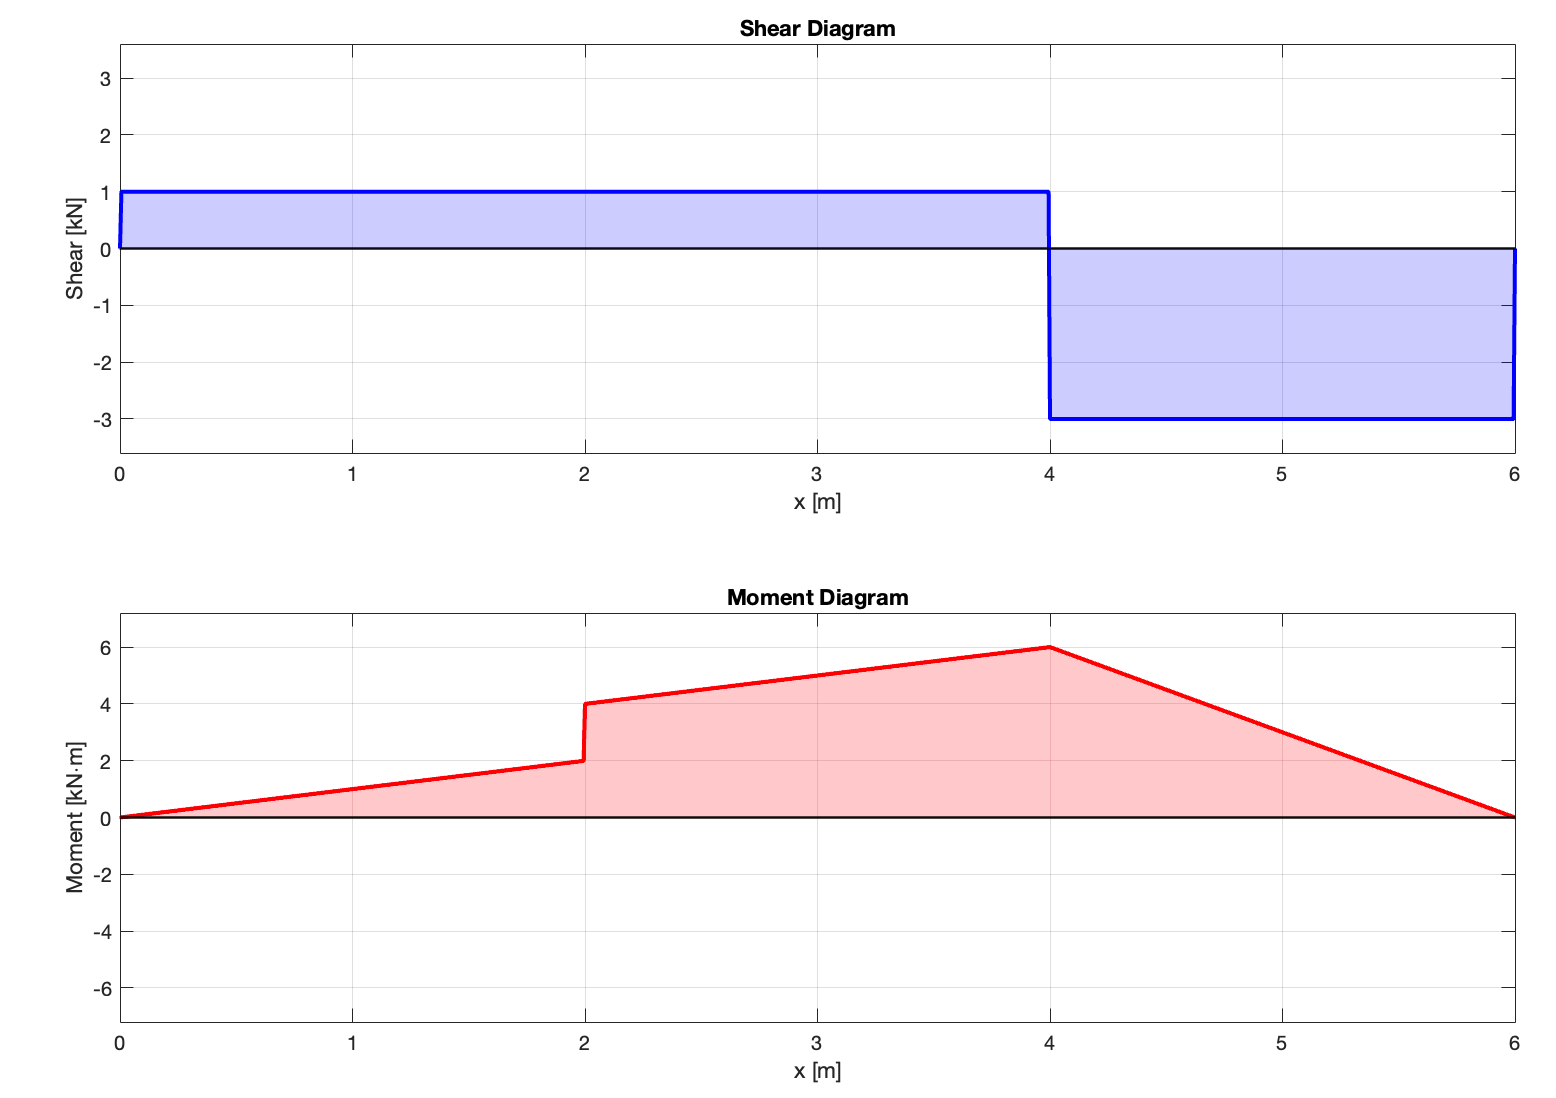
\includegraphics[width=\linewidth]{./figures/f11_18sm.png}
    \caption{Shear and moment diagram for the simply supported beam.}
  \end{figure}
\end{derivation}

\clearpage
